\documentclass[a4paper,12pt]{report}

\usepackage{cmap} % поиск в документе
\usepackage[T2A]{fontenc} % кодировка
\usepackage[utf8]{inputenc} % кодировка исходного текста
\usepackage[english, russian]{babel} % локализация и переносы

\usepackage{hyperref} % гиперссылки
\usepackage{ulem} % перечёркнутый текст
\usepackage{graphicx}  % Для вставки рисунков
\usepackage{indentfirst} % отступ после заголовка
\usepackage[labelsep=period]{caption} % : -> . в caption

\author{Колобов Кирилл, Суслова Диана, Обельченко Иван, 201-321}
\date{}
\title{Аборты: геноцид или выбор?}

\begin{document}
\maketitle
\tableofcontents

\part{За аборты}
\chapter{Позиция}
    Каждый человек имеет право сам решить, хочет он ребёнка или нет.
\chapter{Доводы}
    \section{Зигота -- не человек}
        В физическом смысле зигота не является человеком, это клетка, 
        которая лишь может породить новую жизнь, но только пройдя 
        немалый путь развития.
    \section{Человек начинается с рождения}
        Человеком становятся после рождения, до этого момента момента
        существующий организм называется плодом.
    \section{Зигота -- часть тела матери}
        Эмбрион на ранних стадиях развития не может существовать
        независимо от матери. Законные аборты можно делать на небольшом
        сроке беременности, когда на свет не может появиться живой человек.
    \section{У зиготы нет разума, нет сознания}
        У раннего эмбриона нет разума и сознания.
        У плода на ранних стадиях развития полностью не сформированы многие 
        органы в т.ч. и мозг, он не может мыслить.
    \section{Зигота -- не личность}
        У зиготы не мозга, она ещё не сформировалась, она не 
        личность поэтому её можно убить.
    \section{У женщины есть выбор}
        Женщина имеет право выбирать, как ей распоряжаться своей дальнейшей жизнью. 
        Она хочет убить паразита, чтобы не кормить его и не мучаться.
    \section{Беременность <<по глупости>>}
        Девушка сама ещё ребёнок и беременность не желанна.
        Несовершеннолетние не готовы иметь детей и могут не справиться с ребёнком.
    \section{Она не хотела заводить ребёнка}
        Женщина не хотела заводить ребёнка, она против этого, она ещё не 
        готова поэтому она может сделать аборт.
    \section{Угроза жизни роженицы}
        Роды для женщины могут закончиться даже летальным исходом, 
        а у ребёнка могут быть очень серьёзные физические отклонения.
    \section{По закону можно}
        Какие могут быть вопросы, если законом разрешено?
    \section{А если это было изнасилование?}
        А если это было изнасилование, то тоже нельзя сделать аборт? Женщине рожать ребёнка от насильника?


\chapter{Выводы}
Исходя из всего вышеперечисленного, мы понимаем, что бывают разные ситуации, 
в результате которых женщина может забеременеть. Иногда это может быть не ее 
выбор. Соответственно, она должна иметь право хотя бы самой решить, хочет ли она 
продолжить незапланированную беременность.


\part{Против абортов}
\chapter{Позиция}
Здесь рассматриваются доводы с позиции гипотетической индукции: если можно убить плод, то можно убить 
уже родившегося человека в любом возрасте по тем же причинам, по которым делается аборт,
поскольку качественно человек не меняется с самого момента зачатия, см. пункт \ref{ishuman}.

Однако, сторонники аборотов старательно избегают последовательных рассуждений, 
допуская убийство плода, но выступая против убийства уже рождённых людей, что есть лицемерие,
перетекающее в геноцид.

Часть доказательств в кратком изложении представлены ниже. 

\chapter{Доводы}
    \section{Зигота -- человек}\label{ishuman}
        \begin{figure}[!h]
            \centering
            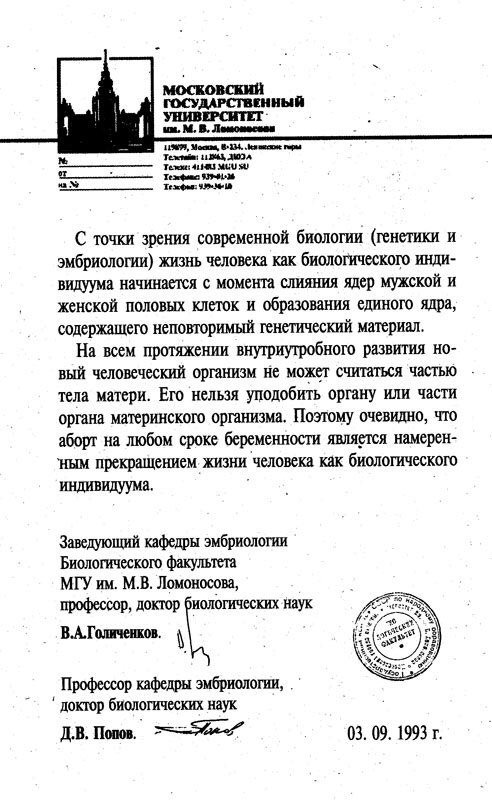
\includegraphics[width=0.45\textwidth]{evidence.jpg}
            \caption{Биологические данные}
        \end{figure}
     
        Человек -- представитель биологического вида \textit{Homo Sapiens Sapiens}, 
        зигота принадлежит к этому виду $\Rightarrow$ зигота -- человек $\Rightarrow$ аборт -- убийство человека.
	\section{Человек начинается с зачатия}
        Зигота -- это первая стадия развития человеческого организма, см. пункт \ref{ishuman}. 
        Любое небиологическое деление -- арбитрарное, не имеет верифицируемых критериев. 

        Невалидность апеляций к законам рассмотрена ниже, пункт \ref{laws}.
	\section{Зигота -- новый организм}
        См. пункт \ref{ishuman}. Зигота -- первая стадия развития человека.

        А также, ребёнок не может жить без матери первые несколько лет после рождения. 
        Однако оппоненты считают, что после рождения убивать нельзя.
        Выходит, этот довод используется непоследовательно, то есть противоречит их позиции.
    \section{Сторонники абортов -- нацисты}\label{nazi}
        В пресуппозициях к таким утверждениям, очевидно, есть следующее положение: 
        <<неразумных>> людей, людей без <<сознания>> можно убивать. 
	    Выходит, сторонники абортов за убийство всех людей с врождёнными или 
        пробритёнными отклонениями: слабоумие, старческая деменция, микроцефалия, 
        анэнцефалия\footnote{Отсутствие больших полушарий.}, вегетативная 
        кома\footnote{Состояние, из которого нельзя выйти, поскольку мозг 
        мёртв. Человек становится овощем.}. 
        Выходит, они не против убийства своей бабушки из-за \sout{жажды наследства} 
        её деменции на почве возраста. Это ли не нацизмом называется?
        
        Вообще говоря, из-за несформировавшегося мозга зигота не перестаёт относиться к 
        биологическому виду \textit{Homo Sapiens Sapiens}, то есть не перестаёт быть человеком.
    \section{А как проверить?}
        У этого параметра нет критериев верификации, аналогично <<сознанию>> из пункта \ref{nazi}.
	\section{Можно убить новорождённого?}
        Если у неё есть выбор, то может ли она убить новорождёного? 
        Если вы считаете, что может, то \sout{вы нацист} аборты, как и любое другое 
        убийство по сиюминутной прихоти, допустимы в рамках ваших ценностей, а 
        если нет -- аборты недопустимы.

        Сторонники абортов против убийства новорождённых, однако не приводят
        доводов, показывающих качественное различие плода и младенца. Иными словами,
        позиция оппонентов непоследовательна.

        Также стоит отметить, что выбор есть всегда. Например, юная девушка 
        могла не шлятся по впискам. Выбор был сделан, это его последствия.
    \section{А чем она думала?}\label{thing-about-it}
        У неё был выбор, она могла отказаться от незащищённого секса. Однако не отказалась, 
        теперь пусть несёт ответственность за свои ошибки. Это не повод убивать кого-то.
	\section{А чем она думала?}
        Аналогично пункту \ref{thing-about-it}.
    \section{Апелляция к едининым случаям}\label{ifdie}
        В цивилизованных странах вероятность осложнений при родах
        (в статистику включены данные о родах 15-летних девушек)
        составляет $ \frac{1}{4900} \approx 0.02\% $, по данным ВОЗ\footnote{https://www.who.int/en/news-room/fact-sheets/detail/maternal-mortality}.

        И если консилиум врачей пришёл к выводу, что роды приведут к 
        смерти роженицы, то это достатоное основание для аборта.
    \section{В III Рейхе...}\label{lawsp}
        Апелляции к законам опять же невалидны, поскольку законы устанавливаются группой 
        людей исходя из их интересов и не могут быть основой человеческой морали. 
	\section{Тогда можно}
        В таком случае аборт допустим, как и в случае угрозы жизни роженицы, пункт \ref{ifdie}.


\chapter{Выводы}
Проблемы абортов, их распространённость и необходимость, у многих наслуху неспроста: 
современному среднечеловеку чуждо чувство отвественности, он не готов ни думать о 
своих действиях заранее, ни принимать последствия совершённых ошибок -- незащищённого 
секса, в данном случае.

Решение этой проблемы неоскорблённые умом видят в массовом геноциде определённой 
группы людей, самых незащищённых из нас --  нерождённых. 

При этом, к сожалению, процесс мышления (как и любовь до гроба, крепкая семья) из 
моды выходит, вследствие этого простая альтернатива гуляет перед лицом у \textit{homo consumer} 
незамеченной. 

Так или иначе, предлагаемая альтернатива решит также проблему неизлечимых (а впрочем, 
излечимых тоже) венирических болезней: ВИЧ, его запущенная форма -- СПИД, 
сифилис, хламидиоз, трихомониаз et cetera.

И альтернатива эта (барабанная дробь!) -- защищённый секс.
\end{document}
